\documentclass{standalone}
\usepackage[svgnames]{xcolor}
\usepackage{tikz}
\usetikzlibrary{arrows.meta}
\begin{document}
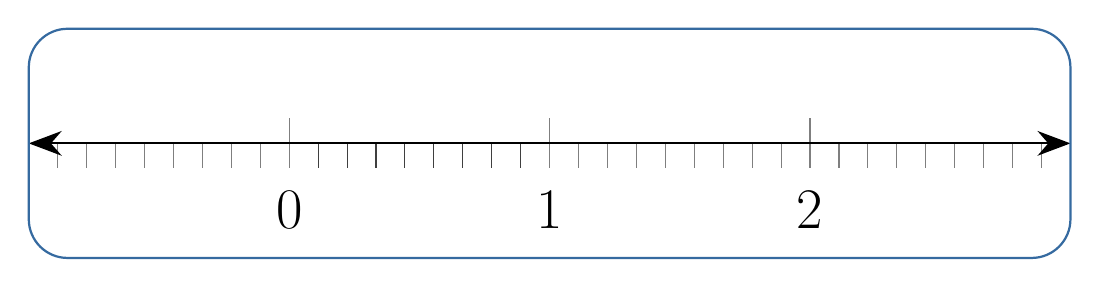
\begin{tikzpicture}[x=1.30208333333333in,y=1.43229166666667in]

\tikzset{
	>={Stealth[scale=1.8]},
	clip even odd rule/.code={\pgfseteorule},
	inverse clip/.style={ clip,insert path=[clip even odd rule]{
		(-1,-0.4) rectangle (3,0.4) }
	}
}
\definecolor{borderblue}{HTML}{356AA0}
\definecolor{fillpurple}{HTML}{A384E5}
\pgfdeclarelayer{background}
\pgfdeclarelayer{foreground}
\pgfsetlayers{background,main,foreground}
\begin{pgfonlayer}{background}
	\fill[white,rounded corners=14pt]
	(-1,-0.4) rectangle (3,0.4);
\end{pgfonlayer}
\huge
\draw[<->,thick] (-1,0) -- (3,0)
node[above left,outer sep=2pt]{\(\)};
\foreach \x/\label in {0/0,1/1,2/2}{\draw[thin, opacity = 0.5] (\x,9pt) -- (\x,-9pt) node[baseline, yshift = -15pt, opacity = 1]{\(\label\)};}
\foreach \x in {-0.888888888888889,-0.777777777777778,-0.666666666666667,-0.555555555555556,-0.444444444444444,-0.333333333333333,-0.222222222222222,-0.111111111111111,0.111111111111111,0.222222222222222,0.333333333333333,0.444444444444444,0.555555555555556,0.666666666666667,0.777777777777778,0.888888888888889,0.111111111111111,0.222222222222222,0.333333333333333,0.444444444444444,0.555555555555556,0.666666666666667,0.777777777777778,0.888888888888889,1.11111111111111,1.22222222222222,1.33333333333333,1.44444444444444,1.55555555555556,1.66666666666667,1.77777777777778,1.88888888888889,2.11111111111111,2.22222222222222,2.33333333333333,2.44444444444444,2.55555555555556,2.66666666666667,2.77777777777778,2.88888888888889}{\draw[thin, opacity = 0.5] (\x,0) -- (\x,-9pt);}
\draw[borderblue,rounded corners=14pt,thick] (-1,-0.4) rectangle (3,0.4);
\begin{pgfonlayer}{foreground}
\clip[rounded corners=14pt] (-1,-0.4) rectangle (3,0.4);
\end{pgfonlayer}
\begin{pgfonlayer}{background}
\end{pgfonlayer}
\end{tikzpicture}
\end{document}
